\documentclass[tikz,border=5pt]{standalone}
\usepackage{tikz}
\usetikzlibrary{arrows.meta,positioning,fit,backgrounds}

\definecolor{promptblue}{HTML}{DCEAF7}
\definecolor{activationgray}{HTML}{E9ECEF}
\definecolor{saegreen}{HTML}{DDEEDF}
\definecolor{graphgold}{HTML}{F6E7C1}
\definecolor{validationrose}{HTML}{F3D9DC}
\definecolor{ink}{HTML}{263238}

\begin{document}
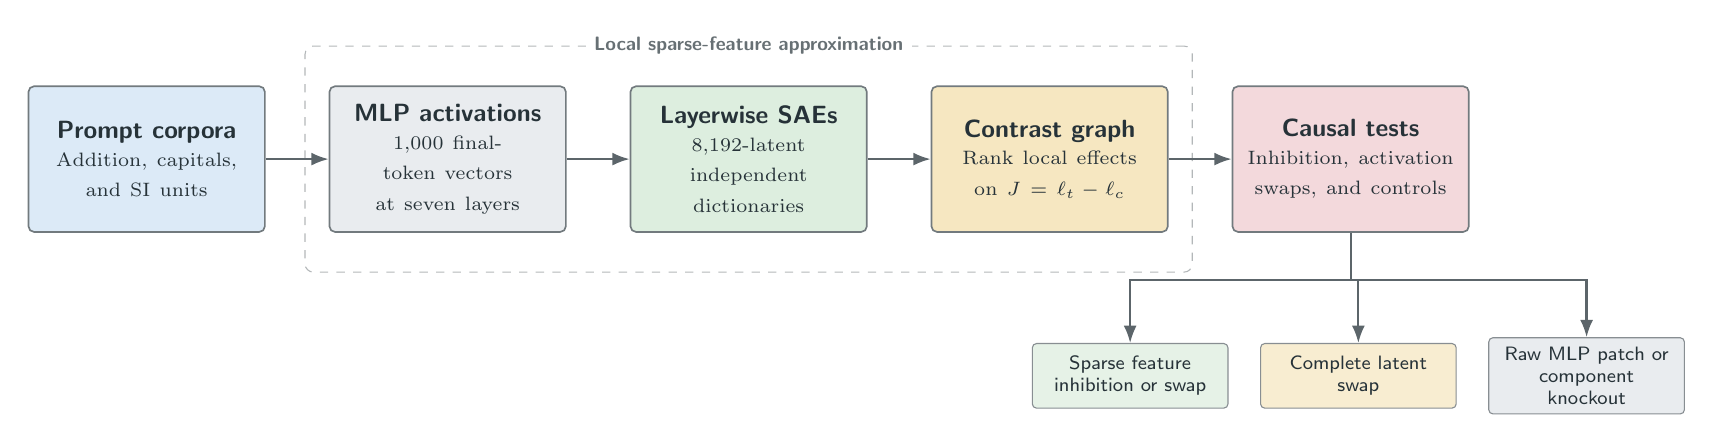
\begin{tikzpicture}[
    font=\sffamily\small,
    text=ink,
    node distance=8mm,
    stage/.style={
        draw=ink!65,
        line width=0.6pt,
        rounded corners=2pt,
        text width=2.65cm,
        minimum height=1.85cm,
        align=center,
        inner sep=5pt,
        font=\sffamily\small\bfseries
    },
    arrow/.style={-{Latex[length=2.2mm]}, line width=0.8pt, draw=ink!75},
    branch/.style={draw=ink!55, rounded corners=1.5pt, text width=2.25cm,
        minimum height=0.82cm, align=center, font=\sffamily\scriptsize},
    grouptext/.style={font=\sffamily\scriptsize\bfseries, text=ink!70,
        fill=white, inner xsep=3pt}
]

\node[stage, fill=promptblue] (prompts) {Prompt corpora\\[-1pt]
    {\normalfont\scriptsize Addition, capitals, and SI units}};
\node[stage, fill=activationgray, right=of prompts] (acts) {MLP activations\\[-1pt]
    {\normalfont\scriptsize 1,000 final-token vectors at seven layers}};
\node[stage, fill=saegreen, right=of acts] (saes) {Layerwise SAEs\\[-1pt]
    {\normalfont\scriptsize 8,192-latent independent dictionaries}};
\node[stage, fill=graphgold, right=of saes] (graph) {Contrast graph\\[-1pt]
    {\normalfont\scriptsize Rank local effects on $J=\ell_t-\ell_c$}};
\node[stage, fill=validationrose, right=of graph] (validation) {Causal tests\\[-1pt]
    {\normalfont\scriptsize Inhibition, activation swaps, and controls}};

\draw[arrow] (prompts) -- (acts);
\draw[arrow] (acts) -- (saes);
\draw[arrow] (saes) -- (graph);
\draw[arrow] (graph) -- (validation);

\node[branch, fill=saegreen!75, below=14mm of validation, xshift=-28mm]
    (sparse) {Sparse feature\\inhibition or swap};
\node[branch, fill=graphgold!75, right=4mm of sparse]
    (latent) {Complete latent\\swap};
\node[branch, fill=activationgray, right=4mm of latent]
    (raw) {Raw MLP patch or\\component knockout};

\coordinate (fork) at ([yshift=-6mm]validation.south);
\draw[arrow] (validation.south) -- (fork) -| (sparse.north);
\draw[arrow] (fork) -| (latent.north);
\draw[arrow] (fork) -| (raw.north);

\begin{scope}[on background layer]
\node[draw=ink!35, dashed, rounded corners=3pt, fit=(acts)(saes)(graph),
      inner xsep=3mm, inner ysep=5mm] (approx) {};
\end{scope}
\node[grouptext] at (approx.north) {Local sparse-feature approximation};

\end{tikzpicture}
\end{document}
